\univlogo

{\Huge April 2}\vspace{5mm}

\section*{Temporary Conclusion}


\subsection*{Conventional droop control}

\begin{figure}[H]
\centering
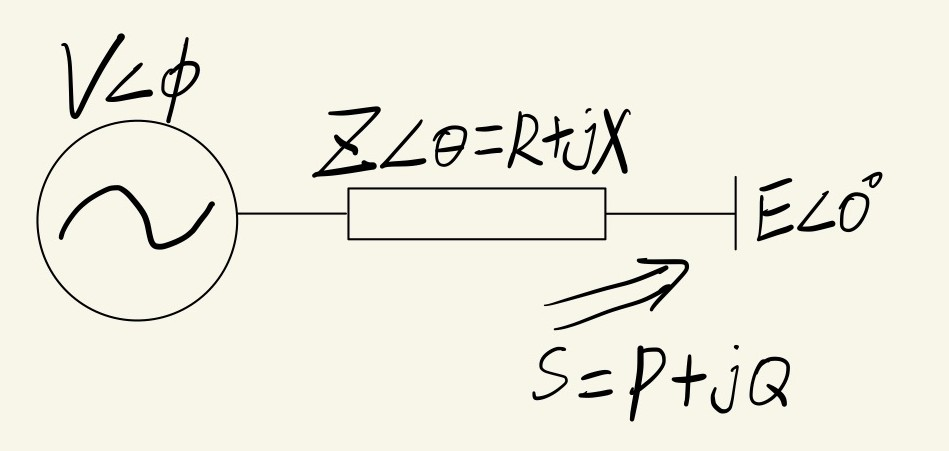
\includegraphics[width=0.6\textwidth]{./2023Mar/SingleInverter.png}
\caption{Single inverter}
\label{Report1SingleInverter}
\end{figure}

When the transmission line is a high voltage line, $X \gg R$, at this time $\theta$ is treated as \textbf{$\cfrac{\pi}{2}$ (purely inductive circuit)}, and the voltage phase angle $\phi$ is relatively small, $\sin{\phi}=\phi$, $\cos{\phi}=1$. The formula can be simplified to:

\begin{equation}
\begin{aligned}
\left\{\begin{array}{l}
    P \doteq \cfrac{EV}{X}\phi    \\
    Q \doteq \cfrac{E}{X}(V-E)
\end{array}\right.
\end{aligned}
\end{equation}

Usually, the voltage angular frequency of the inverter is easier to monitor than the phase angle difference, so the droop control formula can be obtained by substituting the angular frequency for the phase angle difference:

\begin{equation}
\begin{aligned}
\left\{\begin{array}{l}
    \omega = \omega_0-m_pP    \\
    V = V_0 - n_qQ
\end{array}\right.
\end{aligned}
\end{equation}

\subsection*{Phase-Lock Loop}

\begin{figure}[H]
\centering
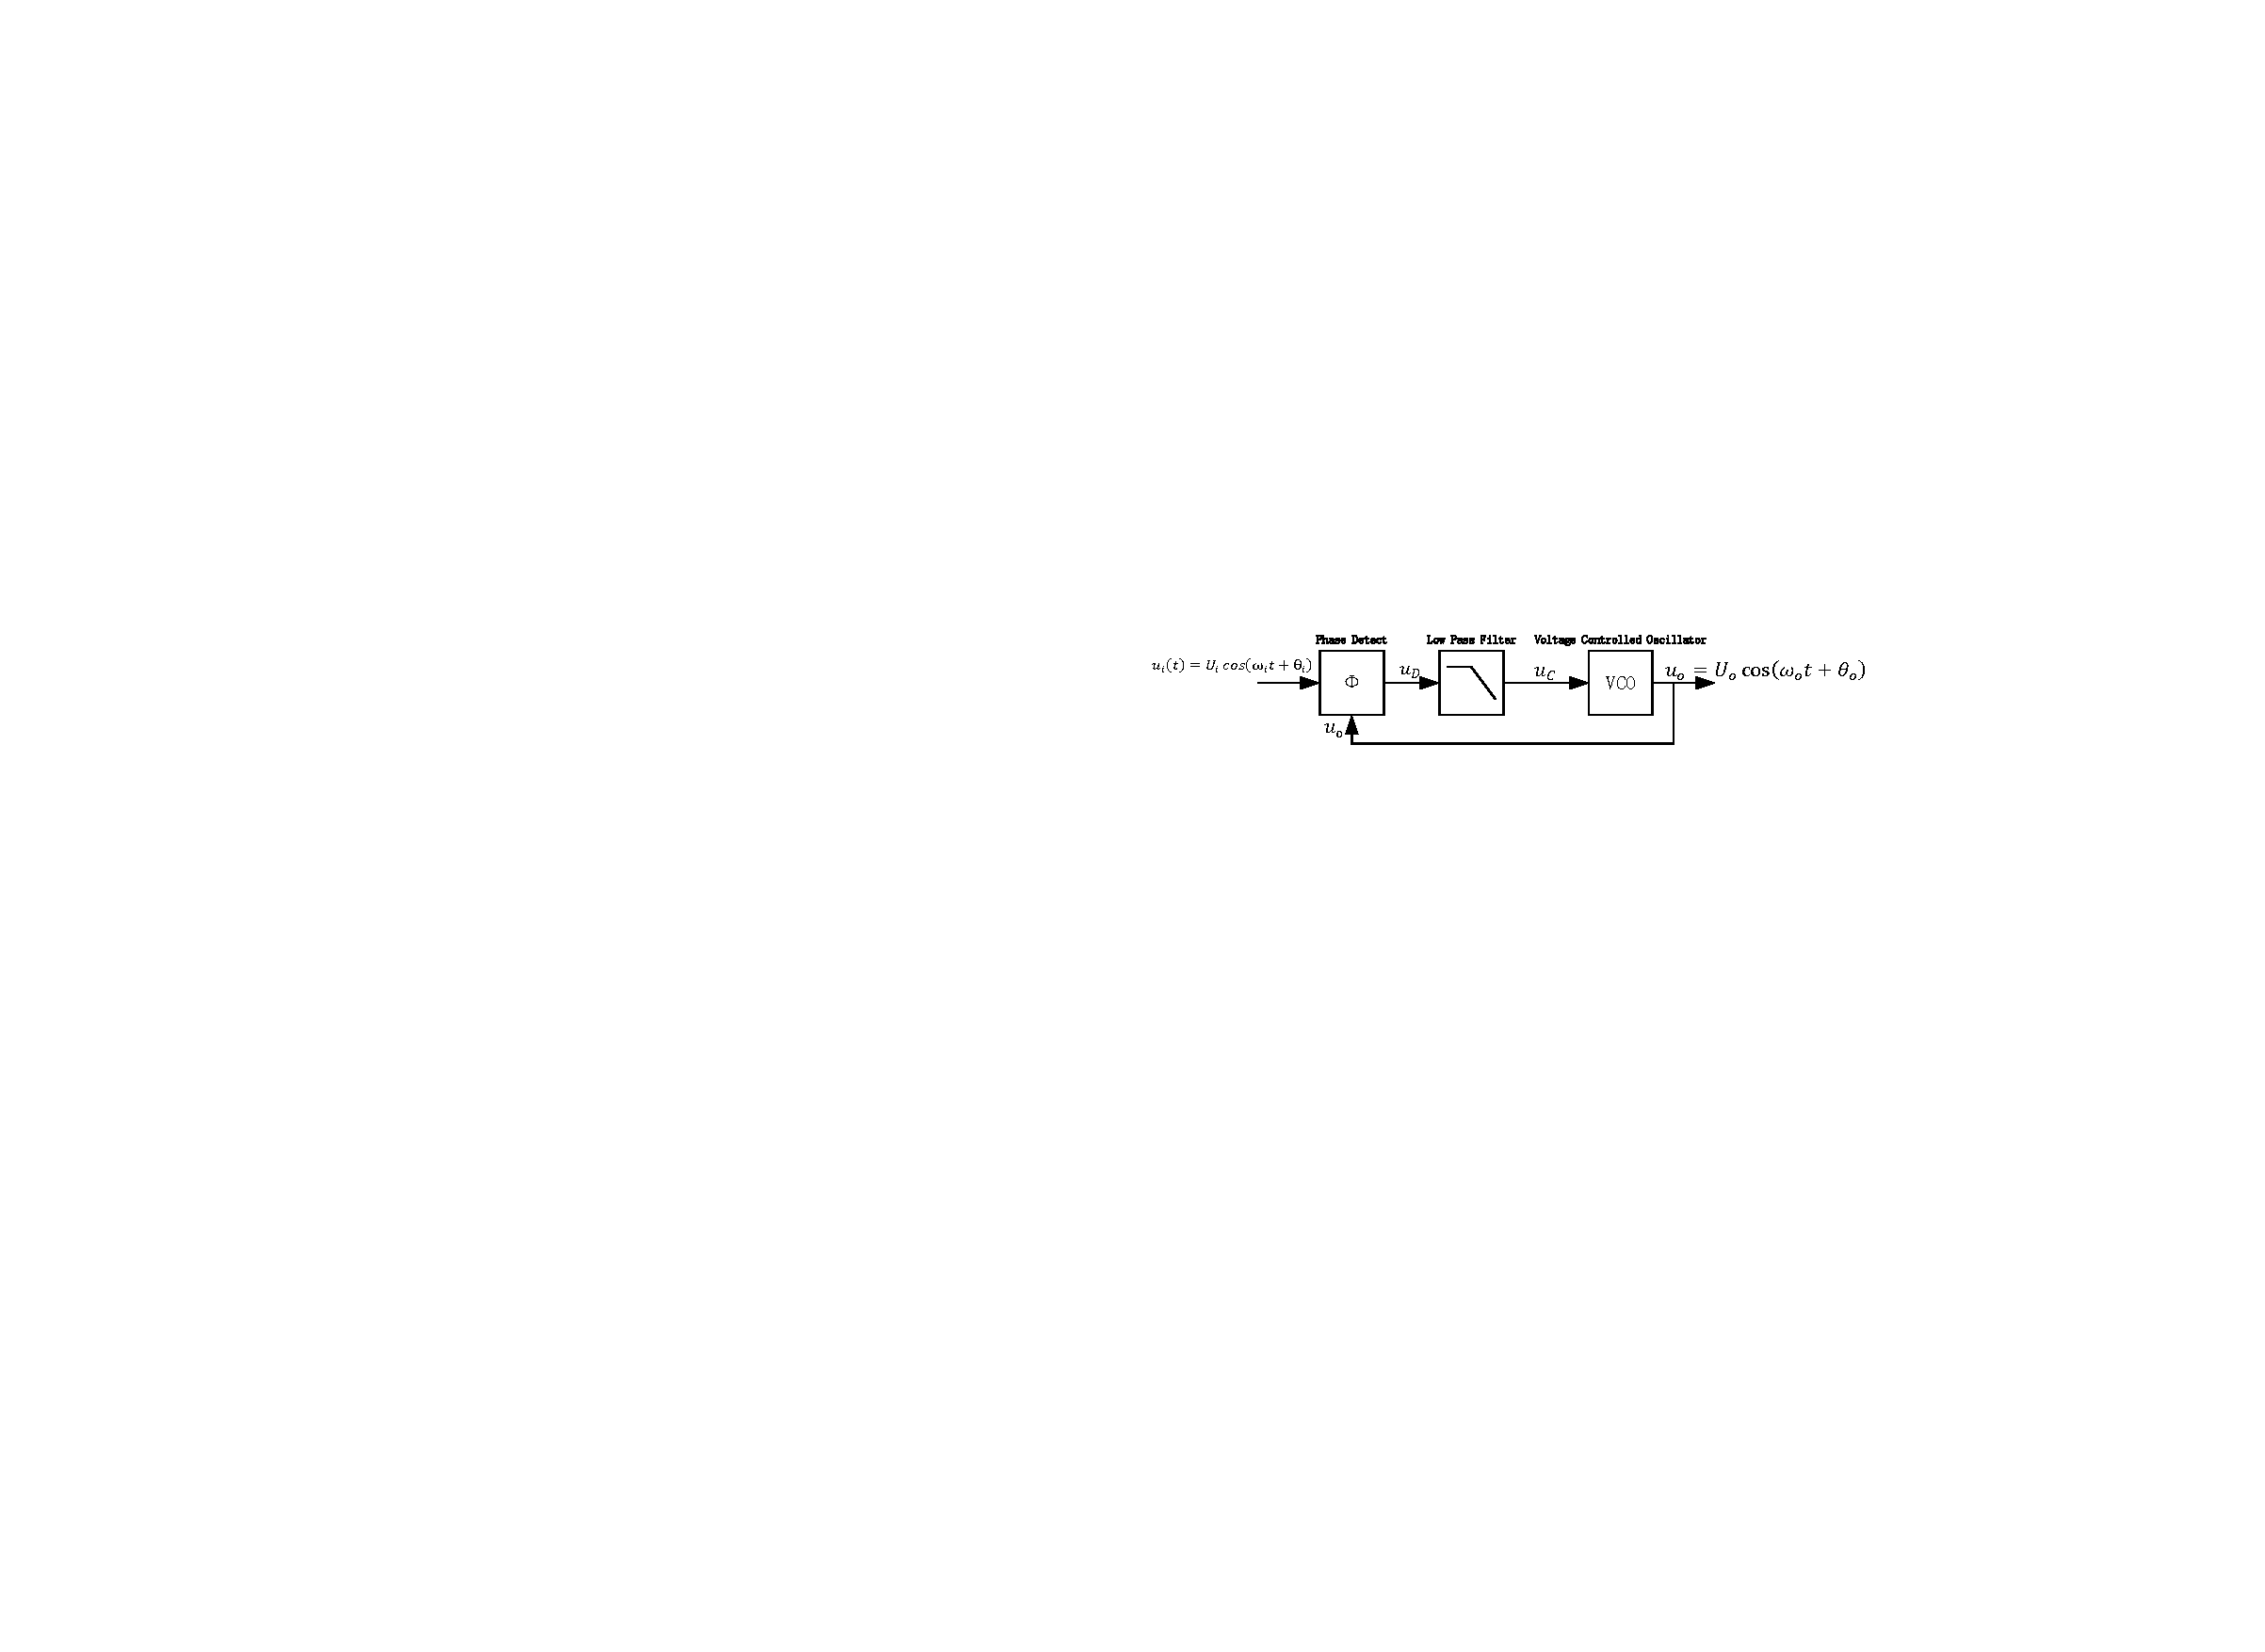
\includegraphics[width=1\textwidth]{./2023Mar/PLL.pdf}
\caption{PLL}
\label{Report1PLL}
\end{figure}

Use PD and LPF to acquire this:

\begin{equation}
\begin{aligned}
    u_C=U_{dm}\cos{((\omega_i-\omega_o)t+(\theta_i(t)-\theta_o(t)))}
\end{aligned}
\end{equation}

The instantaneous frequency expression of this signal $u_C$ is $|\omega_i-\omega_o|$ which can be considered as an error function.

The VCO $\omega_o=K\cos{((\omega_i-\omega_o)t_n+\Delta\theta)}$ will make $\omega_i$ closer to $\omega_o$.

\subsection*{dVOC}

The error function is :


\begin{equation}
\begin{aligned}
    \cfrac{\mathrm{d} v_i}{\mathrm{d} t}=\omega_0Jv_i+\eta e_{\theta,i}(v_i,i_{o,i})+\eta\alpha e_{v,i}(v_i)
\end{aligned}
\end{equation}

where

$\omega_0Jv_i$ is the standard equation of a harmonic oscillator in rectangular coordinates.

\begin{equation}
\begin{aligned}
\left\{\begin{matrix}
    &e_{\theta,i}(v_i,i_{o,i})=K_iv_i-R(k)i_{o,i} &(phase\ error)\\
    &e_{v,i}(v_i)=\phi_i(v_i)v_i &(magnitude\ error)
\end{matrix}\right.
\end{aligned}
\end{equation}

phase error vanishes when the voltage levels and power injections of the inverters corresponds to the setpoints.

magnitude error term vanishes when $v_i^{\star}=\left\|v_i \right\|$

To have $e_{\theta,i}(v_i,i_{o,i})=0$ and $e_{v,i}(v_i)=0$, we need

\begin{equation}
\begin{aligned}
\left\{\begin{array}{l}
    \cfrac{1}{v_i^{\star2}}\begin{bmatrix}
        p_i^\star & q_i^\star\\
        -q_i^\star & p_i^\star
    \end{bmatrix}v_i-i_{0,i}=0\\\\
    v_i^{\star}=\left\|v_i \right\|
\end{array}\right.
\end{aligned}
\end{equation}


There are some matrix operations here, and I'm not sure they can be easily implemented with hardware circuits.

\begin{equation}
\begin{aligned}
\begin{matrix}
   R(k):=
\begin{bmatrix}
    \cos{(k)} & -\sin{(k)}\\
    \sin{(k)} & \cos{(k)}
\end{bmatrix}\\
J:=R(\pi/2)\\
K_i:=\cfrac{1}{v_i^{\star2}}R(k)\begin{bmatrix}
p_i^\star & q_i^\star\\
-q_i^\star & p_i^\star
\end{bmatrix},\ \phi_i(v_i):=\cfrac{v_i^{\star2}-\left\|v_i \right\|^2}{v_i^{\star2}}
\end{matrix}
\end{aligned}
\end{equation}